The next Figure \ref{fig:flow} describes the AI, i.e. the MCTS Algorithm module.

\begin{figure}[H]
	\centering
	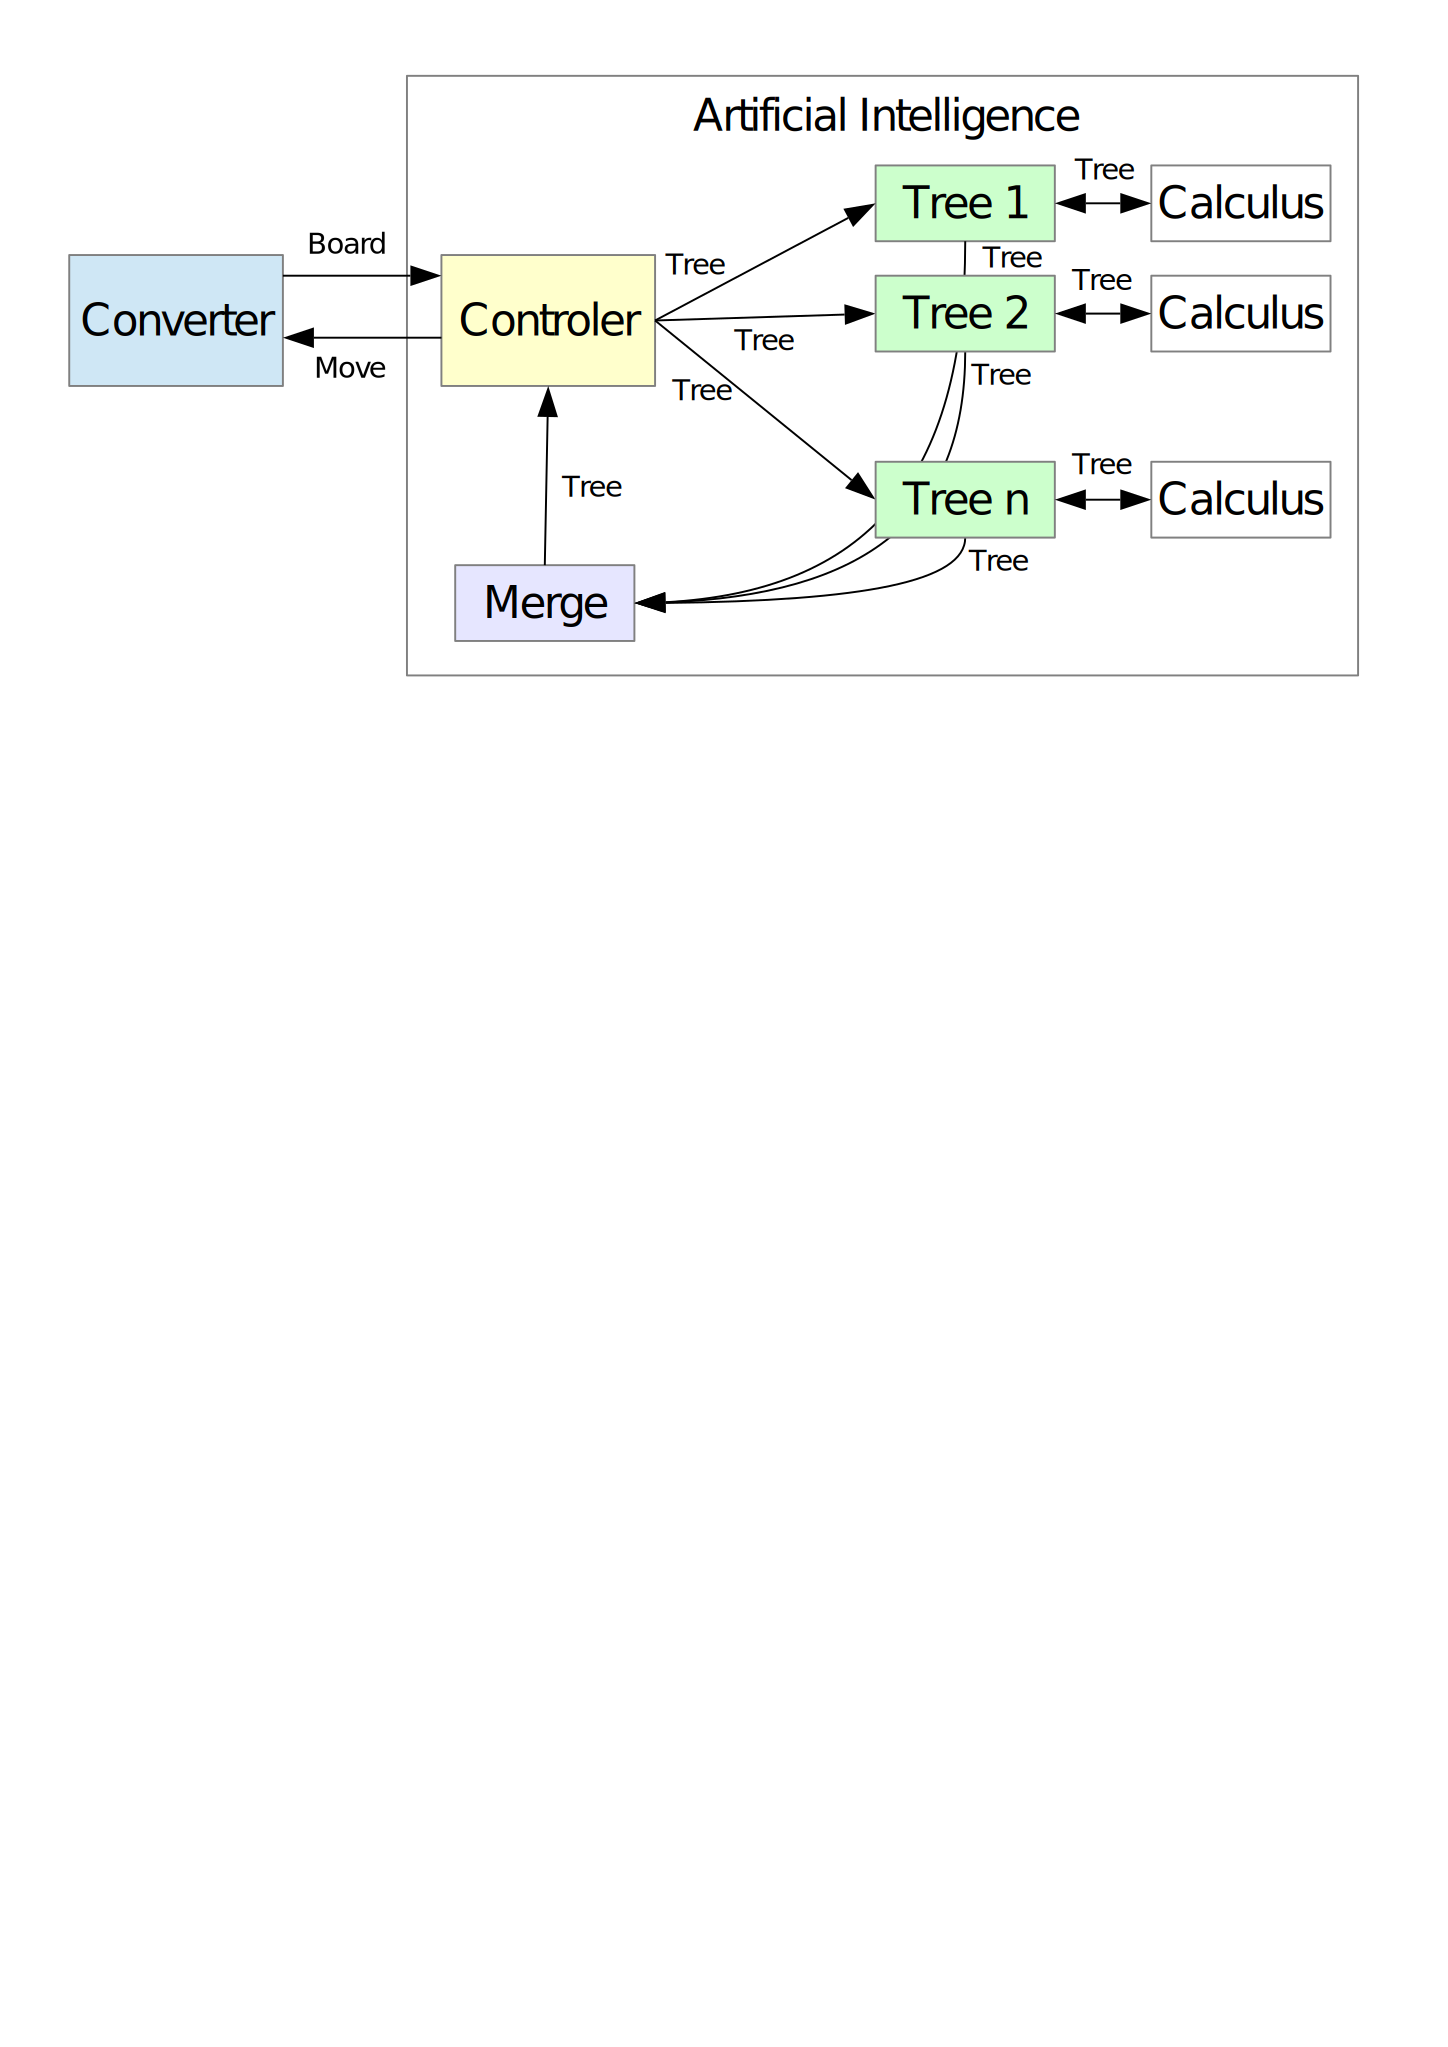
\includegraphics[width=0.80\textwidth]{2General_Architecture/2.3MCTS/AI.jpg}
	\caption{Artificial Intelligence}
	\label{fig:flow}
\end{figure}

The converter sends the state of the board to the controler, which creates trees of moves in different instances of the module. Each of these submodules computes simultaneously his tree, getting the possible moves thanks to a set of rules, represented here by the letter R. Furthermore, these submodules are able to evaluate each chosen move in a tree, comparing winrate and views.

Then, when the calculus is over, the submodules hands over the tree to the Merge module. When all instances of the module have done it, the Merge module merges the trees, gathering data in an only tree, that is sent to the controler.

Finally, the controler is able to decide what move to choose and it sent this move to the converter.

